\documentclass{article}
\usepackage{mathrsfs}
\usepackage{amsmath}
\usepackage{amsthm}
\usepackage{amssymb}
\usepackage{graphicx}
\usepackage{color}
%\include{macros}
%\usepackage{floatflt}
%\usepackage{graphics}
%\usepackage{epsfig}


\theoremstyle{definition}
\newtheorem{theorem}{Theorem}[section]
\newtheorem{lemma}[theorem]{Lemma}
\newtheorem{proposition}[theorem]{Proposition}
\newtheorem{corollary}[theorem]{Corollary}

\theoremstyle{definition}
\newtheorem*{defition}{Definition}
\newtheorem*{example}{Example}

\theoremstyle{remark}
\newtheorem*{remark}{Remark}
\newtheorem*{note}{Note}
\newtheorem*{exercise}{Exercise}

\setlength{\oddsidemargin}{-0.25 in}
\setlength{\evensidemargin}{-0.25 in} \setlength{\topmargin}{-0.25
in} \setlength{\textwidth}{7 in} \setlength{\textheight}{8.5 in}
\setlength{\headsep}{0.25 in} \setlength{\parindent}{0 in}
\setlength{\parskip}{0.1 in}

\newcommand{\homework}[4]{
\pagestyle{myheadings} \thispagestyle{plain}
\newpage
\setcounter{page}{1} \setcounter{section}{#4} \noindent
\begin{center}
\framebox{ \vbox{\vspace{2mm} \hbox to 6.28in { {\bf
THU-70250043,~Pattern~Recognition~(Spring 2016) \hfill Homework: 6} }
\vspace{6mm} \hbox to 6.28in { {\Large \hfill #1 \hfill} }
\vspace{6mm} \hbox to 6.28in { {\it Lecturer: #2 \hfill} }
\vspace{2mm} \hbox to 6.28in { {\it Student: #3 \hfill} }
\vspace{2mm} } }
\end{center}
\markboth{#1}{#1} \vspace*{4mm} }


\begin{document}

\homework{Feature Selection}{Changshui Zhang
\hspace{5mm} {\tt zcs@mail.tsinghua.edu.cn}}{Qingfu Wen \hspace{5mm} {\tt
wqf15@mails.tsinghua.edu.cn } }{8}

%%%%%%%%%%%%%%%%%%%%%%%%%%%%%%%%%%%%%%%%%%%%%%%%%%%%%%%%%%%%%%%%%%%%
% Section 2.  Problem
%%%%%%%%%%%%%%%%%%%%%%%%%%%%%%%%%%%%%%%%%%%%%%%%%%%%%%%%%%%%%%%%%%%%

\section*{Problem 1}\label{problem:1}
\emph{Relation between Fisher Criterion and Least Squares}

It's interesting to see that under some circumstances, the fisher criterion can be obtained as a special case of least squares.
Consider the binary classification problem, let's unify the expression at the very beginning for convenience of the following steps.
And you are required to obey the notations given below.

Suppose we have $N_{1}$ points of class $\mathcal{C}_{1}$ and $N_{2}$ of class $\mathcal{C}_{2}$, then the mean vectors of the two classes
are given by:
\begin{eqnarray}
\bold{m}_{1}= \frac{1}{N_{1}}\sum_{n\in \mathcal{C}_{1}}\bold{x}_{n}, \quad\quad\quad \bold{m}_{2} = \frac{1}{N_{2}}\sum_{n\in \mathcal{C}_{2}}\bold{x}_{n}
\end{eqnarray}
In the lecture notes, we have defined \emph{between-class} covariance matrix and \emph{within-class} covariance matrix:
\begin{eqnarray}
S_{B}=(\bold{m}_{2}-\bold{m}_{1})(\bold{m}_{2}-\bold{m}_{1})^{T}, \quad\quad\quad S_{W}=\sum_{n\in \mathcal{C}_{1}}(\bold{x}_{n}-\bold{m}_{1})(\bold{x}_{n}-\bold{m}_{1})^{T}+\sum_{n\in \mathcal{C}_{2}}(\bold{x}_{n}-\bold{m}_{2})(\bold{x}_{n}-\bold{m}_{2})^{T}
\end{eqnarray}
Now, let's turn to the least square problem. We take the targets for $\mathcal{C}_{1}$ to be $N/N_{1}$ and $\mathcal{C}_{2}$ to be $-N/N_{2}$ where $N=N_{1}+N_{2}$(This may be a little confusing, but you will see the reasons of doing so in a short time). Then the sum-of-square error function can be written as:
\begin{eqnarray}
E=\frac{1}{2}\sum_{n=1}^{N}(\bold{w^{T}}\bold{x}_{n}+w_{0}-t_{n})^2
\end{eqnarray}
Where, $(\bold{x}_{n}, t_{n})$ are the points we have. Target $t_{n}$ equals to $N/N_{1}$ or $-N/N_{2}$ according to its class. Our goal is to estimate $\bold{w}$ and $w_{0}$.

1.1 Show that the optimal $w_{0}$ is: $w_{0}=-\bold{w}^{T}\bold{m}$.
\\
Set
\[\frac{\partial E}{\partial w_{0}}=\sum_{n=1}^{N}(\bold{w^{T}}\bold{x}_{n}+w_{0}-t_{n})=0\]
we got
\begin{equation}\nonumber
\begin{aligned}
w_{0} &= \frac{1}{N}\sum_{n=1}^{N}(t_{n}-\bold{w^{T}}\bold{x}_{n})\\
&= \frac{1}{N}\sum_{n=1}^{N}(t_{n}- \bold{w^{T}}\bold{m})\\
&= \frac{1}{N}(\sum_{n\in\mathcal{C}_{1}}\frac{N}{N_1}+\sum_{n\in\mathcal{C}_{2}}-\frac{N}{N_2}) - \bold{w^{T}}\bold{m}\\
&= -\bold{w^{T}}\bold{m}
\end{aligned}
\end{equation}

1.2 Derive the equation that the optimal $\bold{w}$ should obey:
\begin{eqnarray}
(S_{W}+\frac{N_{1}N_{2}}{N}S_{B})\bold{w}=N(\bold{m_{1}}-\bold{m_{2}})
\end{eqnarray}

Set
\begin{equation}\nonumber
\begin{aligned}
\frac{\partial E}{\partial \bold{w}}=\sum_{n=1}^{N}(\bold{w^{T}}\bold{x}_{n}+w_0-t_{n})x_n&=0\\
\sum_{n=1}^{N}(\bold{w^{T}}\bold{x}_{n}+w_0)x_n-\sum_{n=1}^{N}t_{n}x_n&=0\\
(S_{W}+\frac{N_{1}N_{2}}{N}S_{B})\bold{w}-N(\bold{m_{1}}-\bold{m_{2}})&=0
\end{aligned}
\end{equation}
Thus
\begin{eqnarray}\nonumber
(S_{W}+\frac{N_{1}N_{2}}{N}S_{B})\bold{w}=N(\bold{m_{1}}-\bold{m_{2}})
\end{eqnarray}

1.3 Show me that $\bold{w}$ satisfies: $\bold{w}\varpropto S_{W}^{-1}(\bold{m_{2}}-\bold{m_{1}})$ from equation (4), which means we've got the same form as that of fisher criterion.

\emph{\textbf{SOLUTION:}}\\
$\because S_B\bold{w}=(\bold{m}_{2}-\bold{m}_{1})(\bold{m}_{2}-\bold{m}_{1})^{T}\varpropto (\bold{m_{2}}-\bold{m_{1}})$\\
$\therefore S_W\bold{w}\varpropto (\bold{m_{2}}-\bold{m_{1}})$.\\
Thus,  $\bold{w}\varpropto S_{W}^{-1}(\bold{m_{2}}-\bold{m_{1}})$ .
\\
\section*{Problem 2}\label{problem:2}
\emph{Fisher's discriminant for multiple classes}

Consider the generalization of the Fisher discriminant to $K>2$ classes, and assume that the dimensionality of the input space is greater than the number $K$ of classes. Next, we introduce $D'>1$ linear 'features' $y_{k}=\bold{w}_{k}^{T}\bold{x}$. The weight vectors $\{\bold{w}_{k}\}'s$ can be considered to be the columns of a matrix $\bold{W}$, so that:
\[
\bold{y}=\bold{W}^{T}\bold{x}
\]
Where, $\bold{x}\in \mathcal{R}^{D}$ and $\bold{y} \in \mathcal{R}^{D'}$. By this means, we have projected the $D$-dimensional $\bold{x}$-space onto the $D'$-dimensional $\bold{y}$-space, in which we can better separate the data.

The generalization of the \emph{within-class} covariance matrix to the case of $K$ classes is:
\begin{eqnarray}
S_{W}=\sum_{k=1}^{K}\sum_{n\in \mathcal{C}_{k}}(\bold{x}_{n}-\bold{m}_{k})(\bold{x}_{n}-\bold{m}_{k})^{T}
\end{eqnarray}
Where $\bold{m_{k}}=\frac{1}{N_{k}}\sum_{n\in \mathcal{C}_{k}}\bold{x}_{n}$.

The total covariance matrix is:
\begin{eqnarray}
S_{T}=\sum_{n=1}^{N}(\bold{x}_{n}-\bold{m})(\bold{x}_{n}-\bold{m})^{T}
\end{eqnarray}
Where $\bold{m}=\frac{1}{N}\sum_{n=1}^{N}\bold{x}_{n}=\frac{1}{N}\sum_{k=1}^{K}N_{k}\bold{m}_{k}$.

2.1 Decompose the total covariance matrix $S_{T}$ into \emph{within-class} covariance matrix $S_{W}$ and \emph{between-class} covariance matrix $S_{B}$, and show that $S_{B}$ has the form: $S_{B}=\sum_{k=1}^{K}N_{k}(\bold{m}_{k}-\bold{m})(\bold{m}_{k}-\bold{m})^{T}$
\begin{equation}\nonumber
\begin{aligned}
S_{B}=&S_T-S_W\\
=&\sum_{n=1}^{N}(\bold{x}_{n}-\bold{m})(\bold{x}_{n}-\bold{m})^{T}- \sum_{k=1}^{K}\sum_{n\in \mathcal{C}_{k}}(\bold{x}_{n}-\bold{m}_{k})(\bold{x}_{n}-\bold{m}_{k})^{T}\\
=& \sum_{n=1}^{N}(\bold{x}_{n}\bold{x}_{n}^T-\bold{m}\bold{m}^T)-\sum_{k=1}^{K}\sum_{n\in \mathcal{C}_{k}}(\bold{x}_{n}\bold{x}_{n}^T-\bold{m}_{k}\bold{m}_{k}^T)\\
=& \sum_{k=1}^{K}N_k\bold{m}_{k}\bold{m}_{k}^T-N\bold{m}\bold{m}^T\\
=& \sum_{k=1}^{K}N_k(\bold{m}_{k}-\bold{m})(\bold{m}_{k}-\bold{m})^T
\end{aligned}
\end{equation}
2.2 Write down the \emph{within-class} covariance matrix $s_{W}$ and \emph{between-class} covariance matrix $s_{B}$ of the projected $D'$-dimensional $\bold{y}$-space.
\[s_{W}=\sum_{k=1}^{K}\sum_{n\in \mathcal{C}_{k}}W^T(\bold{x}_{n}-\bold{m}_{k})(\bold{x}_{n}-\bold{m}_{k})^{T}W\]
\[s_{B}=\sum_{k=1}^{K}N_{k}W^T(\bold{m}_{k}-\bold{m})(\bold{m}_{k}-\bold{m})^{T}W\]
2.3 Many possible choices of criterion can be implemented to decide the weight matrix $\bold{W}$, more than 5 examples are shown in Professor Zhang's ppt. Here, we are using another criterion:
\begin{eqnarray}
J(W)=\frac{\Pi_{diag}s_{B}}{\Pi_{diag}s_{W}}
\end{eqnarray}
Where, $\Pi_{diag}A$ means multiplication of the diagonal elements of matrix A.

Represent $J(\bold{W})$ explicitly with $\bold{W}$, $S_{W}$ and $S_{B}$.

\emph{\textbf{SOLUTION:}}\\
\[J(W)=\frac{\Pi_{diag}s_{B}}{\Pi_{diag}s_{W}}= \frac{\Pi_{diag}\bold{W}^TS_{B}\bold{W}}{\Pi_{diag}\bold{W}^T s_{W}\bold{W}}\]

2.4 As is stated above, we now want to project the original data space onto a space with $D'$ dimensions, while at the same time trying to maximize $J(\bold{W})$ represented by equation (7). Write down the equations that columns of weight matrix $\bold{W}$ should obey(which means the selected projection directions).

2.5 As is stated in the problem, we have $K$ classes in all and we are trying to find $D'$ linear 'features'(or projection directions) by maximizing $J(\bold{W})$. How many such 'features' at most are we able to find? Give me your reason.

\section*{Problem 3}\label{problem:3}
\emph{An intuitive understanding between features and error-rates}

Let's review the definition of binary-class Bayesian error-rate at first.

In classification problems, our goal is always to make as few misclassifications as possible. We need a rule that assigns each value of $\bold{x}$ to one of the available classes. Such a rule will divide the input space into regions $\mathcal{R}_{k}$ called \emph{decision regions}, one for each class, such that all points in $\mathcal{R}_{k}$ are assigned to class $\mathcal{C}_{k}$. Take binary classification as an example: A mistake occurs when an input vector belonging to class $\mathcal{C}_{1}$ is assigned to class $\mathcal{C}_{2}$ or vice versa. The error-rate is then given by:
\begin{eqnarray}
p(mistake)=p(\bold{x}\in \mathcal{R}_{1}, \mathcal{C}_{2})+p(\bold{x}\in \mathcal{R}_{2}, \mathcal{C}_{1})\\
=\int_{\mathcal{R}_{1}}p(\bold{x},\mathcal{C}_{2})d\bold{x}+\int_{\mathcal{R}_{2}}p(\bold{x},\mathcal{C}_{1})d\bold{x}
\end{eqnarray}
To minimize the above error-rate, we have to make use of posterior distribution: If $p(\mathcal{C}_{1}|\bold{x})>p(\mathcal{C}_{2}|\bold{x})$, then we assign that $\bold{x}$ to class $\mathcal{C}_{1}$, and vice versa. Thus leading to the Bayesian error-rate.

3.1 Suppose we consider a $K$-class problem, derive the corresponding error rate as that of equation (9).

\emph{\textbf{SOLUTION:}}
\begin{equation}\nonumber
\begin{aligned}
p(mistake)=&\sum_{i=1}^{K}\sum_{j\neq i}\int_{\mathcal{R}_{i}}p(\bold{x},\mathcal{C}_{j})d\bold{x}\\
=&\sum_{i=1}^{K}(1-\int_{\mathcal{R}_{i}}p(\bold{x},\mathcal{C}_{i})d\bold{x})
\end{aligned}
\end{equation}
3.2 Let $x_{i}, i=1, 2, 3$ be independent binary-valued features, and $P(x_{i}=1|w_{1})=\alpha_{i}$, $P(x_{i}=1|w_{2})=\beta_{i}$, $P(w_{1})=P(w_{2})$. Assume that $\beta_{1}-\alpha_{1}>\beta_{2}-\alpha_{2}>\beta_{3}-\alpha_{3}$ and $\alpha_{i}<\beta_{i}$, $\forall i=1, 2, 3$.

Prove that the Bayesian error-rates with only one feature will satisfy $e(x_{1})<e(x_{2})<e(x_{3})$. Give me your explanation of this phenomenon based on the three features.

\emph{\textbf{SOLUTION:}}\\
$P(w_1)=P(w_2)=0.5$,$P(x_i=1)=P(x_{i}=1|w_{1})P(w_2)+P(x_{i}=1|w_{2})P(w_2)=0.5*(\alpha_i+\beta_i)$\\
$P(w_1|x_{i}=1)=\frac{P(w_1,x_i=1)}{P(x_i=1)}=\frac{0.5*\alpha_i}{0.5*(\alpha_i+\beta_i)}=\frac{\alpha_i}{\alpha_i+\beta_i}$
,$P(w_2|x_{i}=1)=\frac{\beta_i}{\alpha_i+\beta_i}$.\\
$P(w_1|x_{i}=0)=\frac{1-\alpha_i}{2-\alpha_i-\beta_i}$,
$P(w_2|x_{i}=0)=\frac{1-\beta_i}{2-\alpha_i-\beta_i}$.\\
The classification criterion is if it belongs to $w_2$ when $x_i=1$, otherwise, it belongs to $w_1$.\\
\begin{equation}\nonumber
\begin{aligned}
e(x_i) =& P(w_1|x_{i}=1)P(x_{i}=1)+P(w_2|x_{i}=0)P(x_{i}=0)\\
=& \frac{\alpha_i}{2}+\frac{1-\beta_i}{2} \\
=& \frac{1-(\beta_i-\alpha_i)}{2}
\end{aligned}
\end{equation}
Since $\beta_{1}-\alpha_{1}>\beta_{2}-\alpha_{2}>\beta_{3}-\alpha_{3}$, $e(x_1)<e(x_2)<e(x_3)$.\\
For only one feature, the feature with largest $\beta_i-\alpha_i$ has lowest error rate.

3.3 With the following parameters:
\[
\alpha_{1}=0.1,\qquad \alpha_{2}=0.05,\qquad \alpha_{3}=0.01
\]\[
\beta_{1}=0.9,\qquad \beta_{2}=0.8,\qquad \beta_{3}=0.7
\]
Calculate $e(x_{1})$, $e(x_{2})$, $e(x_{3})$; $e(x_{1}, x_{2})$, $e(x_{1}, x_{3})$, $e(x_{2}, x_{3})$. Compare the values of different error-rates and present your explanation from the view of feature selection.

\emph{\textbf{SOLUTION:}}\\
$e(x_1)=\frac{1-(0.9-0.1)}{2}=0.1$,$e(x_2)=\frac{1-(0.8-0.05)}{2}=0.125$,$e(x_3)=\frac{1-(0.7-0.01)}{2}=0.155$.\\
$P(w_1,x_i=1,x_j=1)=\alpha_i\alpha_j$,$P(w_1,x_i=1,x_j=0)=\alpha_i(1-\alpha_j)$.\\
$P(w_1,x_i=0,x_j=1)=(1-\alpha_i)\alpha_j$,$P(w_2,x_i=0,x_j=0)=(1-\beta_i)(1-\beta_j)$.\\
$e(x_1,x_2)=0.1*0.05+0.1*0.95+0.9*0.05+0.2*0.1=0.165.$\\
$e(x_1,x_3)=0.1*0.01+0.1*0.99+0.9*0.01+0.1*0.3=0.139.$\\
$e(x_2,x_3)=0.05*0.01+0.05*0.99+0.95*0.01+0.2*0.3=0.1195.$\\
Since $e(x_1)<e(x_2,x_3)<e(x_2)<e(x_1,x_3)<e(x_3)<e(x_1,x_2)$, we can see that feature selection is not easy to handle.
\section*{Problem 4: Programming}
\emph{Fisher discriminant on the ORL Database of Faces}

In this task, you are required to cope with the ORL Database of Faces, which contains a set of face images. This is a famous database, there are ten different images of each of 40 distinct persons. An \emph{orl\_faces.mat} file is provided, with a $400\times 4096$ matrix \emph{data} and a $400\times 1$ vector \emph{label}. Each row of \emph{data} corresponds to a face, you can view the i-th face by matlab command "\emph{imshow(uint8(reshape(data(i, :), 64, 64)))} ". Each element of \emph{label} ranges from 1 to 40, indicating the person's id.

4.1 Use Fisher's linear discriminant with "one-versus-one" strategy and Fisher's discriminant for multiple classes discussed in $\bold{Problem 2}$ to reduce the dimensions of the feature space separately(The original feature space is 4096).

\emph{Hint: The standard fisher linear discriminant is based on binary-class problem, so each round we implement this criterion, we will get an optimal direction $\bold{w}$ determined by class $\mathcal{C}_{i}$ and class $\mathcal{C}_{j}$. Thus, "one-versus-one" strategy means that we should implement fisher linear discriminant on every two classes: since we have 40 classes in all, this strategy will lead to $C_{40}^{2}=780$ binary discriminant functions in total. Each point is then classified according to a majority vote amongst the discriminant functions. But if your laptop is slow in the computation of matrix inverse, you can just experiment on 10 of the 40 classes.}

\emph{\textbf{SOLUTION:}}\\
I don't know how to reduce the dimension using "one-versus-one" strategy and only implemented Fisher's discriminant for multiple classes, you may see the matlab code of \texttt{fisherLDA.m}.

4.2 Design a classifier based on the new feature space.

\emph{Hint: Recall what you have learned in the previous lectures, you now have a few choices of classifiers such as softmax regression, bayesian inference, SVM and KNN. With this course going on, you'll learn more classifiers, our suggestion for you is to keep these methods in mind and become more skilled at them.}

\emph{\textbf{SOLUTION:}}\\
Based on Fisher's linear discriminant analysis above, I implemented kNN(k=3) and SVM(linear kernel) classifiers for new feature space with different dimension. The table below shows classification accuracy of two classifiers.
\begin{table}[!htbp]
\centering
\begin{tabular}{|c|c|c|c|}
\hline
 dim & kNN & SVM  \\
\hline
 $1$ & $0.925$ & $0.9875$  \\
\hline
 $2$ & $0.925$ & $0.9875$  \\
\hline
$4$&$ 0.925 $& $0.9875$  \\
\hline
$8$ & $0.925$ & $0.9875$  \\
\hline
$16$ & $0.925$ & $0.9875$ \\
\hline
$32$ & $0.925$ & $0.9875$\\
\hline
$64$ & $0.925$ & $0.9875$\\
\hline
$128$ & $0.925$ & $0.9875$\\
\hline
$256$ & $0.925$ & $0.9875$\\
\hline
$512$ & $0.925$ & $0.9875$\\
\hline
\end{tabular}
\caption{Classification accuracy of different dimension}
\end{table}

4.3 Discuss the results and compare the two strategy of reducing data dimensions. What's more, the "one-versus-one" strategy may lead to some ambiguous results, you can illustrate this fact with some simple hand-drawn images.
\begin{figure}
\centering
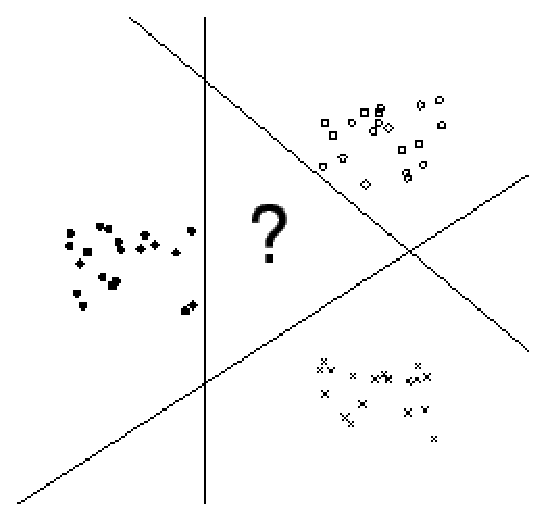
\includegraphics[width=4.5cm]{ovo.eps}
\caption{"one-versus-one" strategy}
\label{fig:fig}
\end{figure}
\emph{\textbf{SOLUTION:}}\\
From figure \ref{fig:fig}, we can see that "one-versus-one" strategy may have some unknown area that does not belong to any classes.
\section*{Problem 5: Programming}
\emph{Feature selection with L1-norm regularization}

This programming task seems to be heavy, but don't be afraid. This is actually an easy work as long as you follow the steps and hints provided.

In this problem, let's consider a regularized approach to feature selection in a simple regression context. Unlike fisher criterion, we are not going to reduce dimensions, but just select features from the existed ones. Suppose we have training inputs $X=(\bold{x}_{1},...,\bold{x}_{n})^{T}$ and corresponding outputs $\bold{y}=(y_{1},...,y_{2})^{T}$, where $\bold{x}_{i}\in \mathcal{R}^{D}$ and $y_{i}\in \mathcal{R}$. We want to train a linear predictor $\hat{y}(\bold{x};\bold{w})=\bold{w}^{T}\phi(\bold{x})$ with $\phi(\bold{x})$ indicating the $M$ features $\phi(\bold{x})=(\phi_{1}(\bold{x}),...,\phi_{M}(\bold{x}))^{T}$. The objective is regularized least-squares as following:
\begin{eqnarray}
J(\bold{w};\lambda)=\frac{1}{n}\sum_{i=1}^{n}\frac{1}{2}(y_{i}-\bold{w}^{T}\phi(\bold{x}_{i}))^{2}+\lambda||\bold{w}||_{1}
\end{eqnarray}
Where $||\bold{w}||_{1}$ is the L1-norm:
\begin{eqnarray}
||\bold{w}||_{1}=\sum_{k=1}^{M}|w_{k}|
\end{eqnarray}
Thus, our task is to minimize the regularized objective in order to seek for the optimal parameters $\hat{\bold{w}}=\hat{\bold{w}}(\lambda)$:
\begin{eqnarray}
\hat{\bold{w}}=arg min_{\bold{w}\in\mathcal{R}^{M}}J(\bold{w};\lambda)
\end{eqnarray}
Implementation of the L1-norm will lead to a sparse $\bold{w}$. What's more, with $\lambda$ increasing, more elements of weight vector $\bold{w}$ are forced to zero, which means the corresponding features are ignored in the predictor.

\emph{Coordinate descent} will be used to solve this L1-regularized least-squares problem. In this approach, we adjust one parameter at a time so as to minimize the objective while keeping the remaining parameters fixed:
\begin{eqnarray}
\hat{w}_{k}=argmin_{w_{k}}J(\bold{w};\lambda)
\end{eqnarray}
With $k$ iterating over all indices \{1,...,M\}, and repeating the process for many times, parameter $\bold{w}$ asymptotically converges to the global minimum of the convex objective (Not familiar with definition of convex? wiki or google).

Since the L1 regularization is not smooth, we can't take derivatives as the differentiable functions to minimize the objective. Instead, we make use of the \emph{subdifferential of a convex function}, which is defined as:
\begin{eqnarray}
\partial f(w)=\{s|f(w+\Delta)\geq f(w)+s\Delta, \forall \Delta\in\mathcal{R}\}
\end{eqnarray}
This is a set-valued generalization of the normal derivative and reduces to the normal derivative $\partial f(w)=\{\frac{\partial f(w)}{\partial w}\}$ whenever $f$ is differentiable. Taking the absolute value function $f(w)=|w|$ as an example:
\begin{displaymath}
\partial f(w)= \left\{ \begin{array}{ll}
\{-1\}, & \textrm{$w<0$} \\
$[-1, +1]$, & \textrm{$w=0$} \\
\{+1\}, & \textrm{$w>0$}
\end{array} \right.
\end{displaymath}
We will use the following result from non-smooth analysis:

$\bold{Optimality}$ $\bold{Condition}$: $\hat{w}$ is a global minimizer of a convex function $f(w)$ if and only if $0\in \partial f(\hat{w})$.

For example, the optimality condition $0 \in \partial f(w)$ for the absolute value function $f(w)=|w|$ holds if and only if $w=0$. Hence, $w=0$ is the unique global minimizer of $|w|$.

Below, we will guide you through the analysis to solve the L1-norm regularized least-squares problem.

5.1 Show that the sub-differential of $J(\bold{w};\lambda)$ with respect to parameter $w_{k}$ is:
\begin{displaymath}
\partial_{w_{k}}J(\bold{w};\lambda)=(a_{k}w_{k}-c_{k})+\lambda\partial_{w_{k}}|w_{k}| =\left\{ \begin{array}{ll}
\{a_{k}w_{k}-(c_{k}+\lambda)\}, & \textrm{$w_{k}<0$} \\
$[-$c_{k}$-$\lambda$, -$c_{k}$+$\lambda$]$, & \textrm{$w_{k}=0$} \\
\{a_{k}w_{k}-(c_{k}-\lambda)\}, & \textrm{$w_{k}>0$}
\end{array} \right.
\end{displaymath}
With:
\begin{eqnarray}
a_{k}=\frac{1}{n}\sum_{i=1}^{n}\phi_{k}^{2}(\bold{x}_{i})
\end{eqnarray}
\begin{eqnarray}
c_{k}=\frac{1}{n}\sum_{i=1}^{n}\phi_{k}(\bold{x}_{i})(y_{i}-\bold{w}_{-k}^{T}\phi_{-k}(\bold{x}_{i}))
\end{eqnarray}
Where $\bold{w}_{-k}$(respectively $\phi_{-k}$) denote the vector of all parameters (features) except for parameter $w_{k}$ (feature $\phi_{k}$). Observe equations (15) and (16), you can find that $a_{k}$'s are non-negative and constant parameters while each $c_{k}$ depends on all parameters except for the parameter $w_{k}$ that we are to update. Try to interpret the coefficient $c_{k}$.

\emph{\textbf{SOLUTION:}}\\
\begin{equation}\nonumber
\begin{aligned}
J(\bold{w};\lambda)&=\frac{1}{n}\sum_{i=1}^{n}\frac{1}{2}(y_{i}-\bold{w}^{T}\phi(\bold{x}_{i}))^{2}+\lambda||\bold{w}||_{1}\\
&=\frac{1}{n}\sum_{i=1}^{n}\frac{1}{2}(y_{i}-\bold{w}_{-k}^{T}\phi_{-k}(\bold{x}_{i})-w_k\phi_{k}(\bold{x}_{i}))^{2}+\lambda||\bold{w}||_{1}\\
&=\frac{1}{n}\sum_{i=1}^{n}\frac{1}{2}\left[(y_{i}-\bold{w}_{-k}^{T}\phi_{-k}(\bold{x}_{i}))^{2}-2w_k\phi_{k}(\bold{x}_{i})(y_{i}-\bold{w}_{-k}^{T}\phi_{-k}(\bold{x}_{i}))+w_k^2\phi_{k}^2(\bold{x}_{i})\right]+\lambda||\bold{w}||_{1}\\
&=\frac{1}{n}\sum_{i=1}^{n}\frac{1}{2}(y_{i}-\bold{w}_{-k}^{T}\phi_{-k}(\bold{x}_{i}))^{2}-c_kw_k+\frac{1}{2}a_kw_k^2+\lambda||\bold{w}||_{1}\\
\end{aligned}
\end{equation}
Thus
\begin{equation}\nonumber
\begin{aligned}
\partial_{w_{k}}J(\bold{w};\lambda)=(a_{k}w_{k}-c_{k})+\lambda\partial_{w_{k}}|w_{k}|
\end{aligned}
\end{equation}
and
\begin{displaymath}
\partial_{w_{k}}|w_{k}|= \left\{ \begin{array}{ll}
\{-1\}, & \textrm{$w_{k}<0$} \\
$[-1, +1]$, & \textrm{$w_{k}=0$} \\
\{+1\}, & \textrm{$w_{k}>0$}
\end{array} \right.
\end{displaymath}
Finally
\begin{displaymath}
\partial_{w_{k}}J(\bold{w};\lambda)=(a_{k}w_{k}-c_{k})+\lambda\partial_{w_{k}}|w_{k}| =\left\{ \begin{array}{ll}
\{a_{k}w_{k}-(c_{k}+\lambda)\}, & \textrm{$w_{k}<0$} \\
$[-$c_{k}$-$\lambda$, -$c_{k}$+$\lambda$]$, & \textrm{$w_{k}=0$} \\
\{a_{k}w_{k}-(c_{k}-\lambda)\}, & \textrm{$w_{k}>0$}
\end{array} \right.
\end{displaymath}

5.2 Solve the non-smooth optimality condition for $\hat{w}_{k}$ s.t. $0 \in \partial_{w_{k}}J(\hat{w_{k}})$. It's helpful to consider each of the following cases separately: \\
\qquad\qquad (a) $c_{k}<-\lambda$\\
\qquad\qquad (b) $c_{k}\in [-\lambda, +\lambda]$\\
\qquad\qquad (c) $c_{k}>+\lambda$\\
In each case, provide a plot $\partial_{w_{k}}J(w_{k})$ versus $w_{k}$ and label the zero-crossing $\hat{w_{k}}$. Then, with the help of those plots, you can express $\hat{w_{k}}$ as a function of $a_{k}$, $c_{k}$ and $\lambda$. Finally, provide a plot of $\hat{w_{k}}$ versus $c_{k}$. What role does the regularization parameter $\lambda$ play in this context relative to the coefficient $c_{k}$ ?

\emph{Hint: There is no need for you to spend too much time generating those plots required above. Since those plots are just small tools helping you understand the final equations. You can just provide me with your hand-drawn plots, either inserted in your report, or included in the codes' folder.}

\emph{\textbf{SOLUTION:}}\\
\begin{figure}
\centering
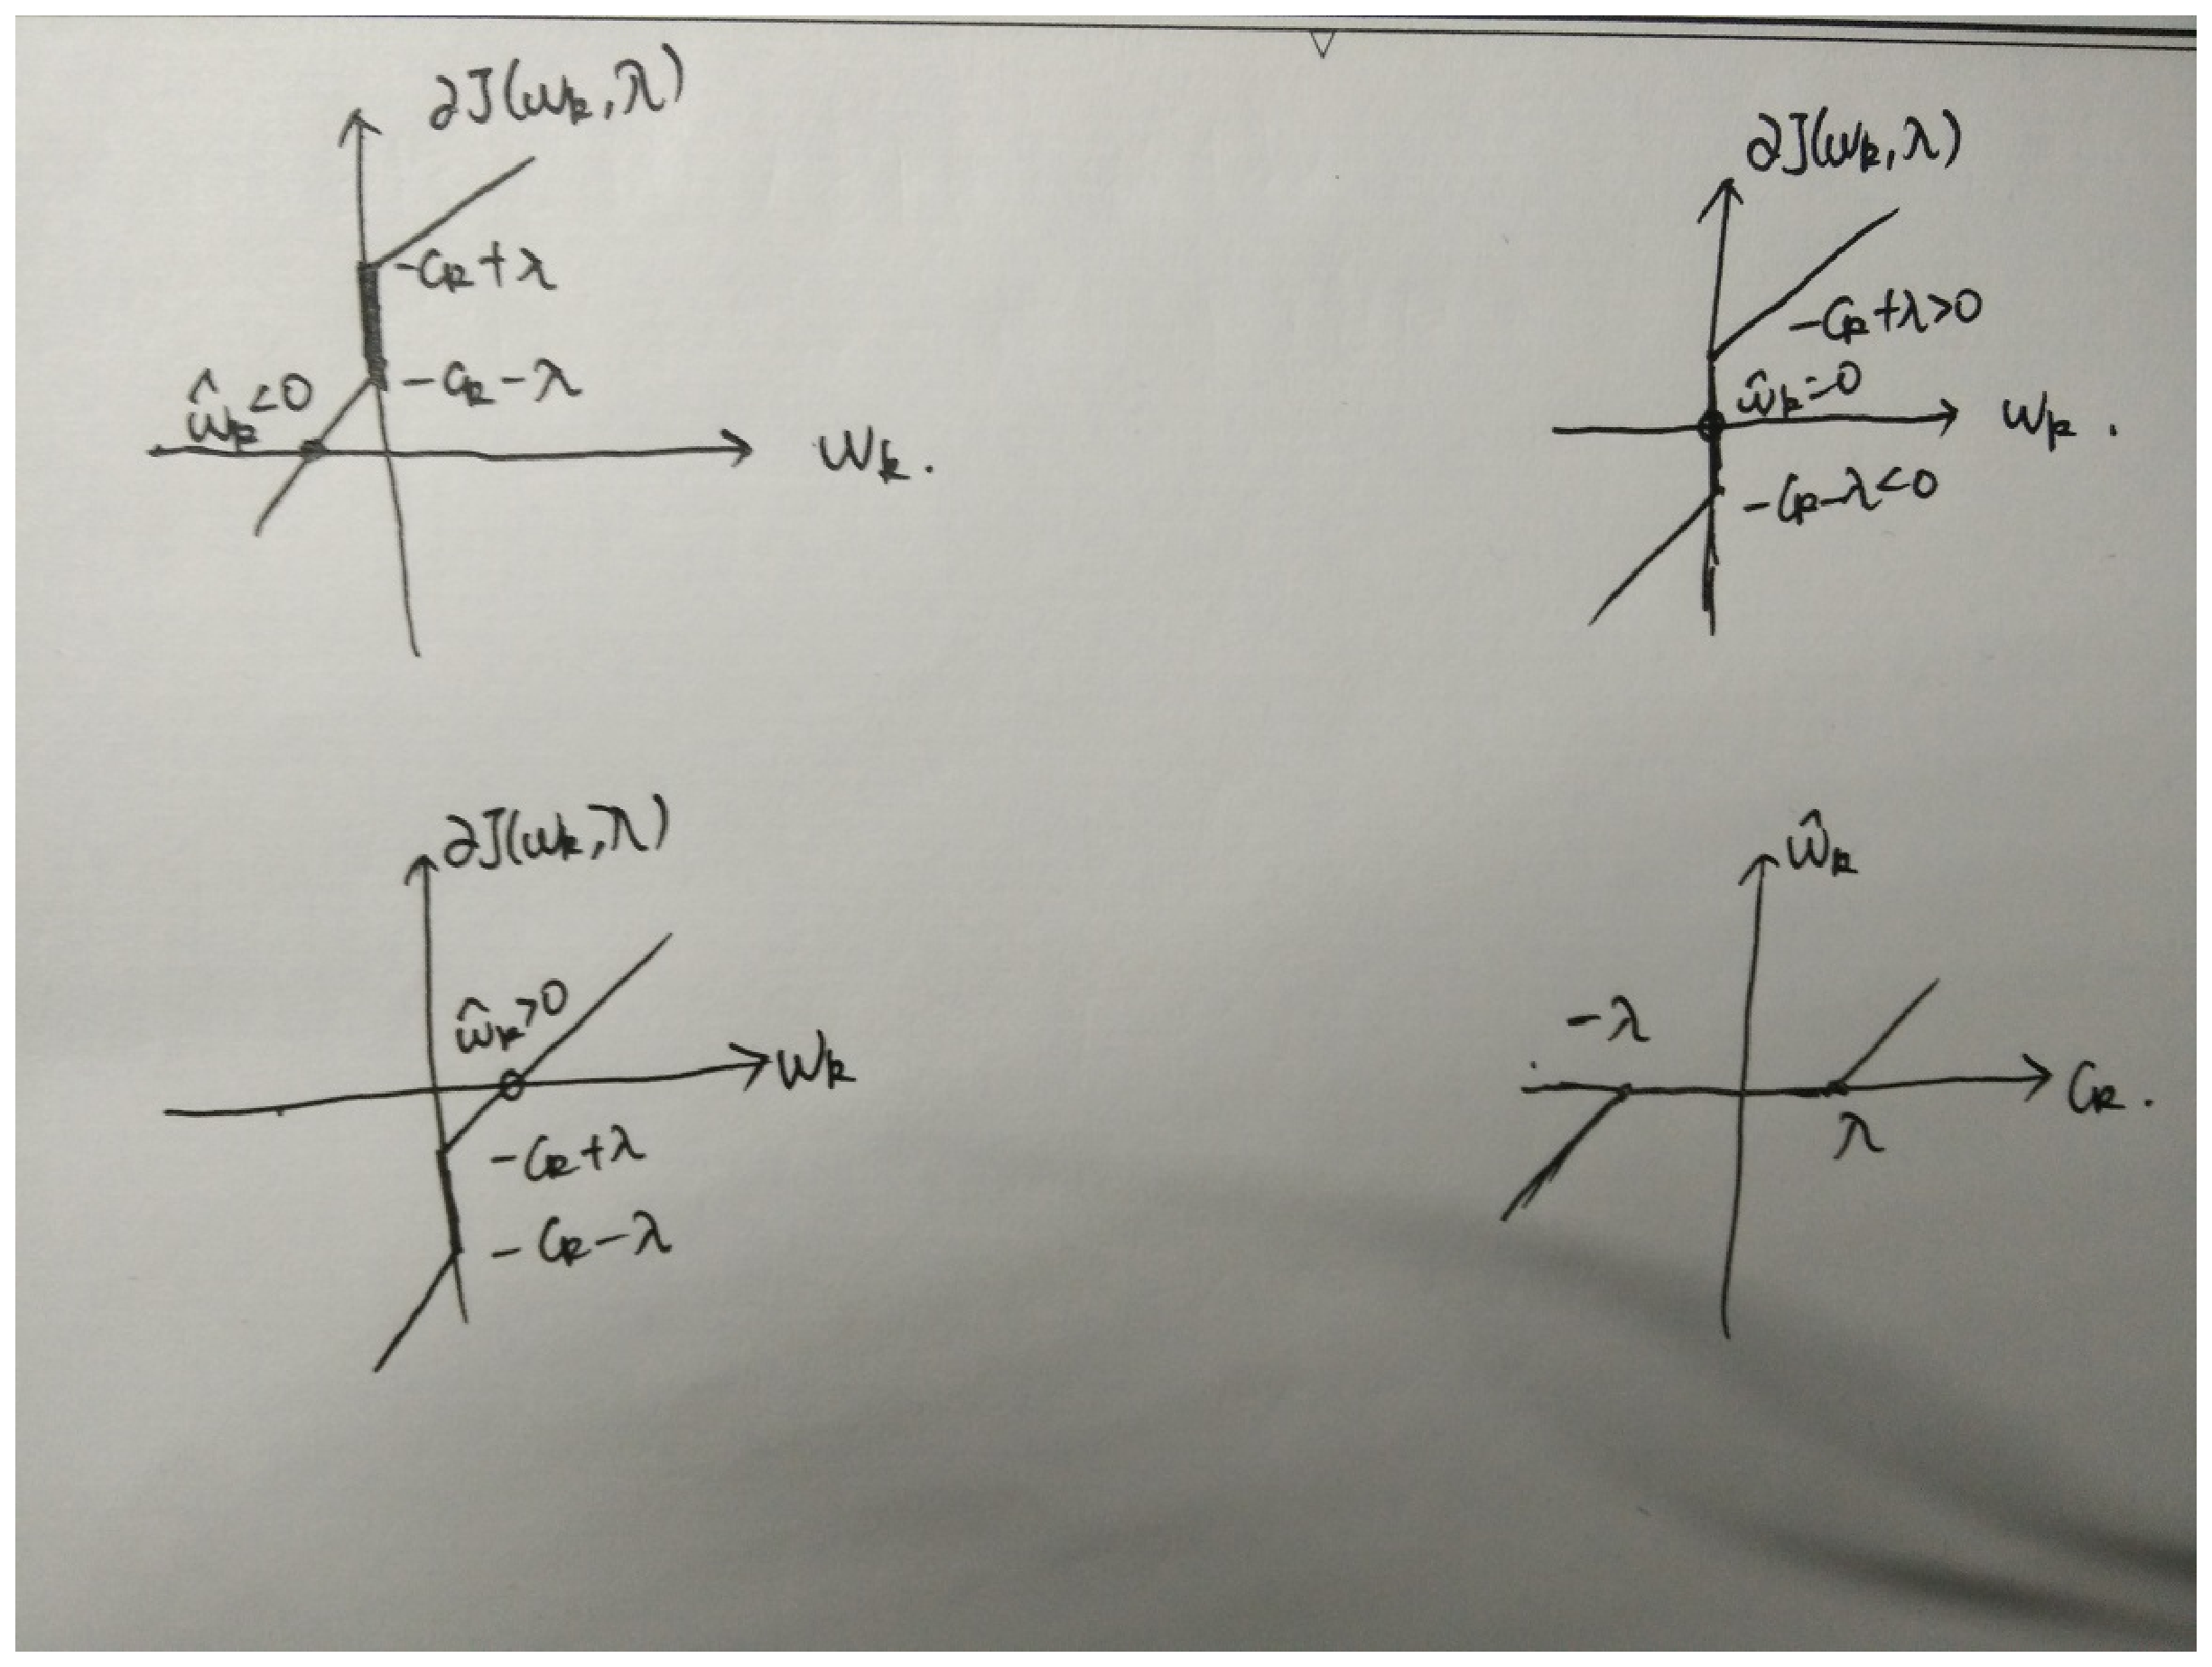
\includegraphics[width=10cm]{wk.eps}
\label{fig:fig}
\end{figure}
\qquad\qquad (a) if $c_{k}<-\lambda$, $c_k+\lambda<0$. By solving $a_{k}w_{k}-(c_{k}+\lambda)=0$, we have
\[\hat{w_k} =\frac{c_{k}+\lambda}{a_k}<0\]\\
\qquad\qquad (b) if $c_{k}\in [-\lambda, +\lambda]$, $-\lambda<c_k<\lambda $. Thus, $\partial_{w_{k}}J(\bold{w};\lambda)$ occurs when
 \[\hat{w_k} =0\]\\
\qquad\qquad (c) if $c_{k}>\lambda$, $-c_k+\lambda<0$. By solving $a_{k}w_{k}-(c_{k}-\lambda)=0$, we have
\[\hat{w_k} =\frac{c_{k}-\lambda}{a_k}>0\]\\
Above all, we can write $w_{k}$ into a function of $c_k$ form.
\begin{displaymath}
\hat{w_k} =\left\{ \begin{array}{ll}
\frac{c_{k}+\lambda}{a_k}, & c_{k}<-\lambda\\
0, & c_{k}\in [-\lambda, +\lambda] \\
\frac{c_{k}-\lambda}{a_k}, & c_{k}>\lambda
\end{array} \right.
\end{displaymath}
we can see that, if $|c_k| < \lambda$,  $w_k$ goes to 0, which means $\mathbf{w}$ is sparse; if $|c_k| > \lambda$, $w_k\neq 0$. Thus, the larger $\lambda$ is, the sparser $\mathbf{w}$ will be.

5.3 We have provided you with training and testing data in the file $\bold{least\_sq.mat}$. Load this file into MATLAB workspace and you will find 4 structures $\bold{test}$, $\bold{train\_large}$, $\bold{train\_mid}$, $\bold{train\_small}$ each containing an $n\times M$ matrix $X$ and a $n\times 1$ vector $\bold{y}$.

For simplicity, we only consider the linear regression, say $\phi(\bold{x})=\bold{x}$. Write a MATLAB subroutine based on the skeleton $\bold{least\_sq\_L1.m}$ to solve for the optimal parameter $\hat{\bold{w}}$ given the training data $(X, \bold{y})$.

\emph{Hint: The skeleton code is just a suggestion, you are not strictly required to follow it as long as you can realize the algorithm.}

\emph{What's more, before writing the code, review the equations derived in 5.2, you may find that the expression for $\hat{w}_{k}$ considered under different cases can be included into just one simple equation, which can accelerate your code by eliminating "if-else" snippets.}

5.4 Complete the skeleton $\bold{mainFunc.m}$ to run your algorithm for a sequence of $\lambda$ values [0.01: 0.01: 2.0]. And we use $\bold{w}_{0}=(X^{T}X)^{-1}X^{T}\bold{y}$, the usual least-squares parameter estimation as the initial state for $\bold{w}$. Also, a function $\bold{least\_sq\_multi.m}$ is provided, you should read the code carefully.

Plot each of the following versus $\lambda$:\\
(a) the training error $J(\hat{\bold{w}}(\lambda);0)$\\
(b) the regularization penalty $||\hat{\bold{w}}(\lambda)||_{1}$\\
(c) the minimized objective $J(\hat{\bold{w}}(\lambda);\lambda)$\\
(d) the number of non-zero parameters $||\hat{\bold{w}}(\lambda)||_{0}$(the L0-norm)\\
(e) the test error

Run this experiment for each of the three training set $\bold{train\_large}$, $\bold{train\_mid}$ and $\bold{train\_small}$, then test on set $\bold{test}$. Comment on the behavior of each of these quantities as a function of $\lambda$. For each training set, what value of $\lambda$ minimizes the test error? How does this vary with the size of the training set? How could we estimate from the training data the appropriate value of $\lambda$ to use so as to approximately minimize the test error?

\emph{Hint: Above all, we've guided you through the basic idea of optimizing the L1-norm problem. L1-regularization is greatly related to the field of compress sensing or sparse representation which was a hot topic for a few years, to learn more, wiki or google.}

\emph{\textbf{SOLUTION:}}\\
we can see that when $\lambda$ increases, the training error increase and regularization penalty consequently decrease.\\
The objective function increases smoothly when $\lambda$ increases.\\
The test error gets local minimum for a certain $\lambda$, with multi-times running of different $\lambda$, we can find the minimum of test error.\\
When $\lambda$ gets larger enough, L0 norm becomes 0, which means $w_k$ is 0. The larger $\lambda$ is, the more 0s are in $\mathbf{w}$.
\begin{figure}[!htbp]
\begin{minipage}[t]{0.3\linewidth}
\centering
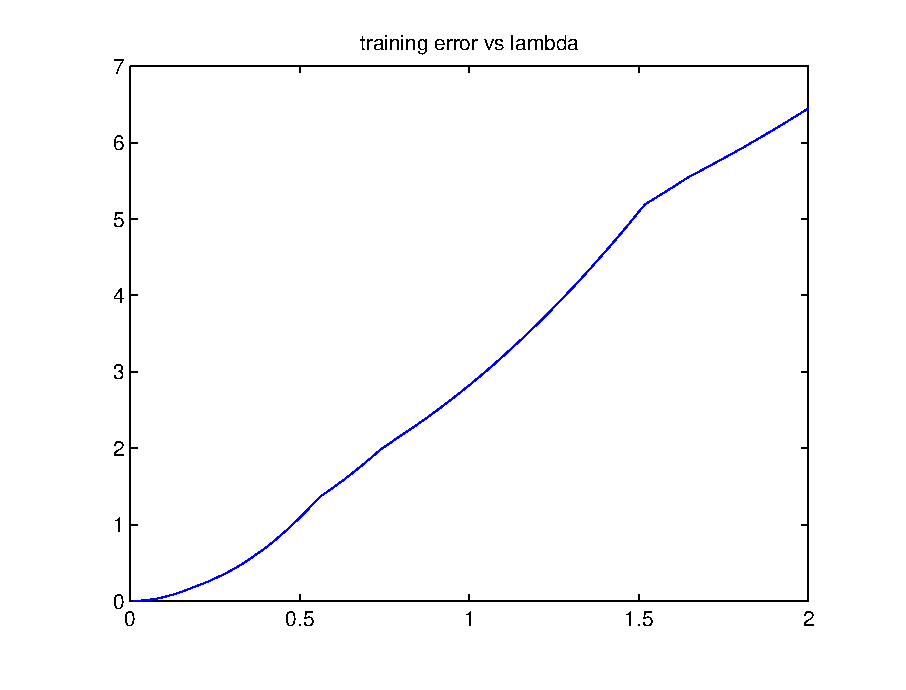
\includegraphics[width=2.2in]{s1.eps}
\end{minipage}%
\begin{minipage}[t]{0.3\linewidth}
\centering
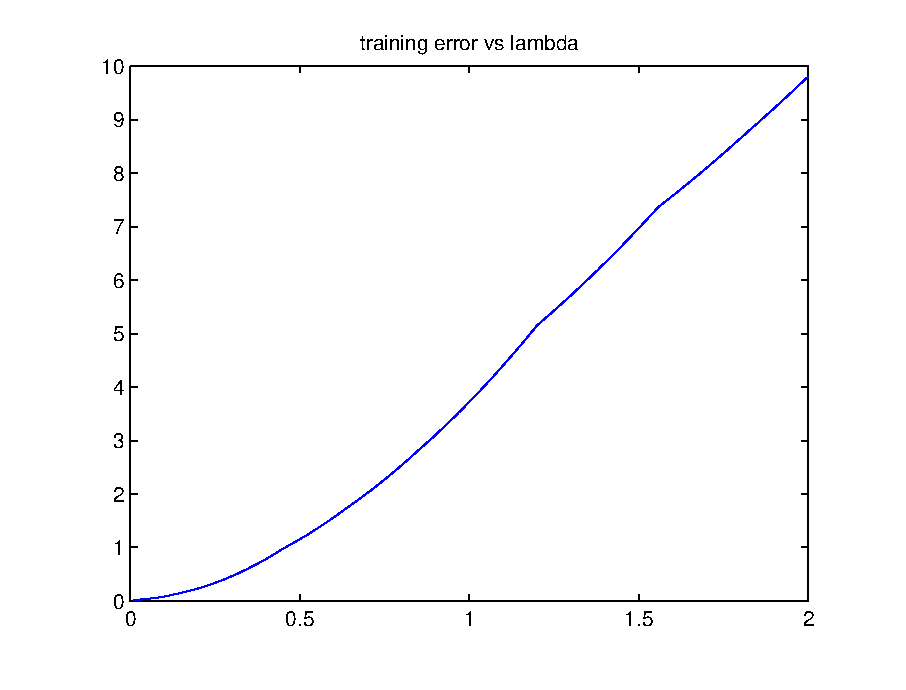
\includegraphics[width=2.2in]{m1.eps}
\end{minipage}
\begin{minipage}[t]{0.3\linewidth}
\centering
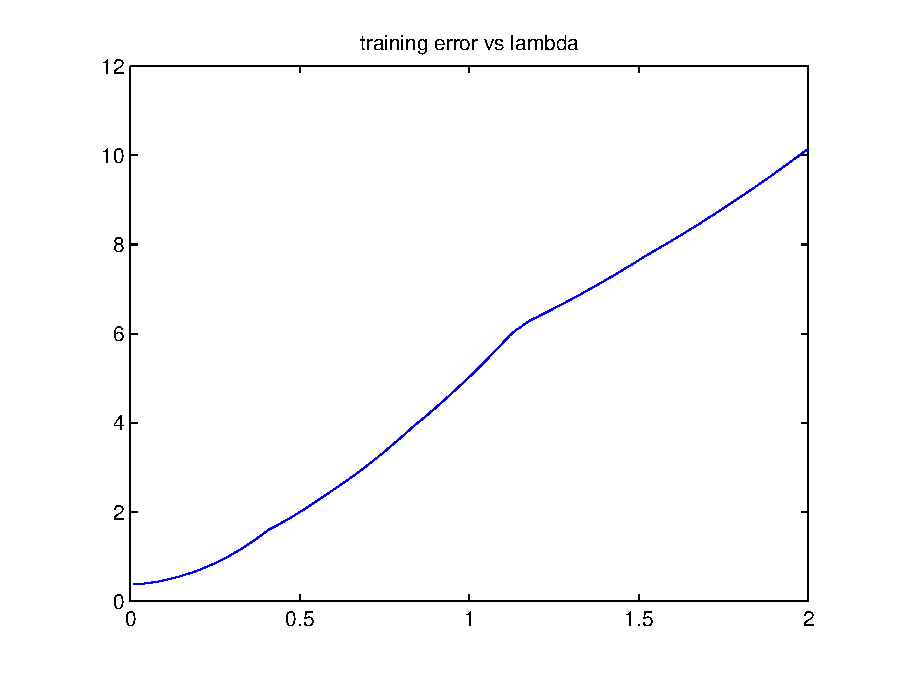
\includegraphics[width=2.2in]{l1.eps}
\end{minipage}
\end{figure}
\begin{figure}[!htbp]
\begin{minipage}[t]{0.3\linewidth}
\centering
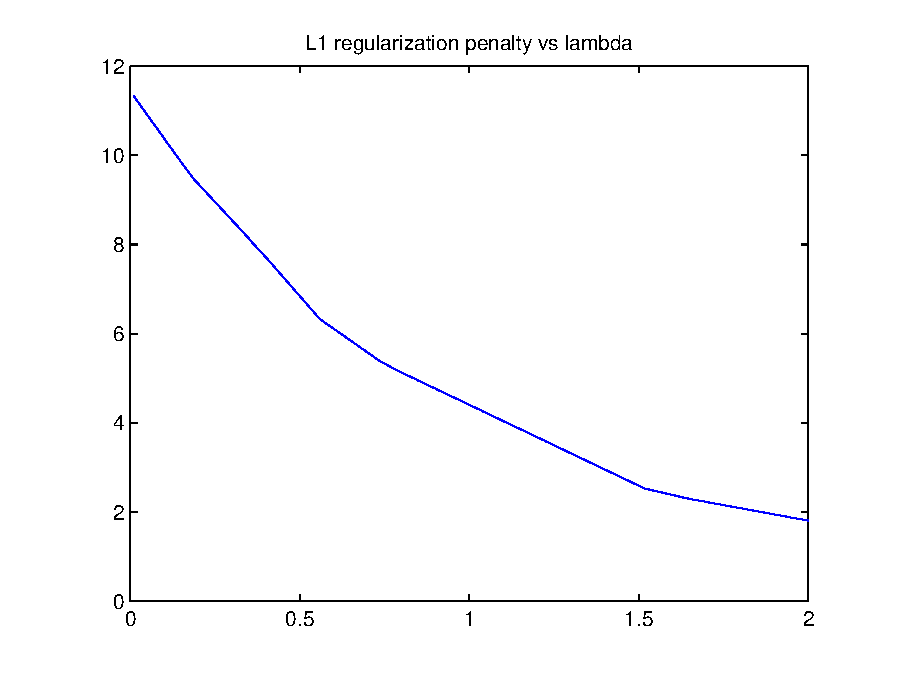
\includegraphics[width=2.2in]{s2.eps}
\end{minipage}%
\begin{minipage}[t]{0.3\linewidth}
\centering
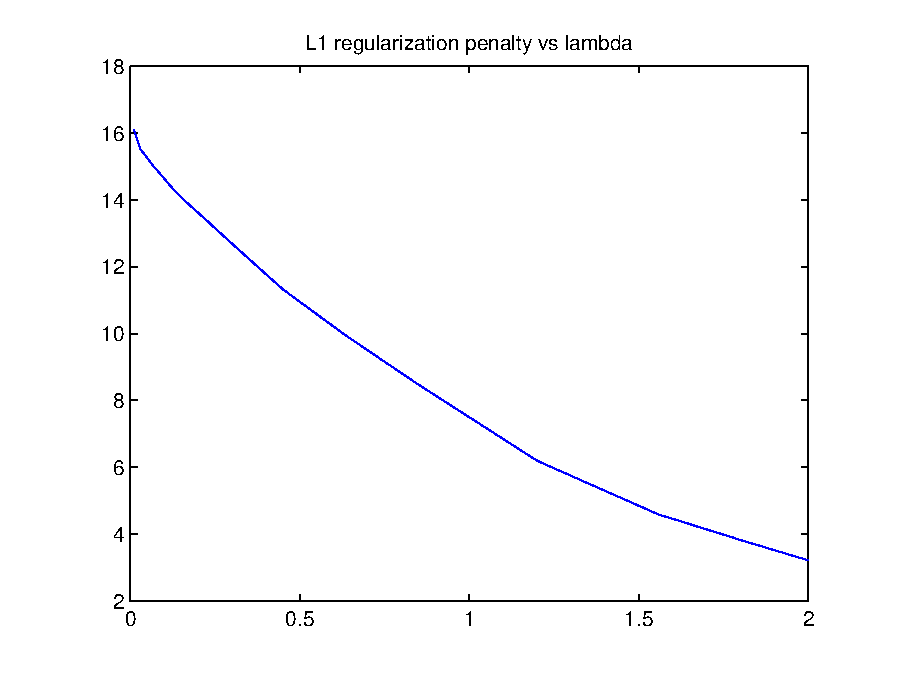
\includegraphics[width=2.2in]{m2.eps}
\end{minipage}
\begin{minipage}[t]{0.3\linewidth}
\centering
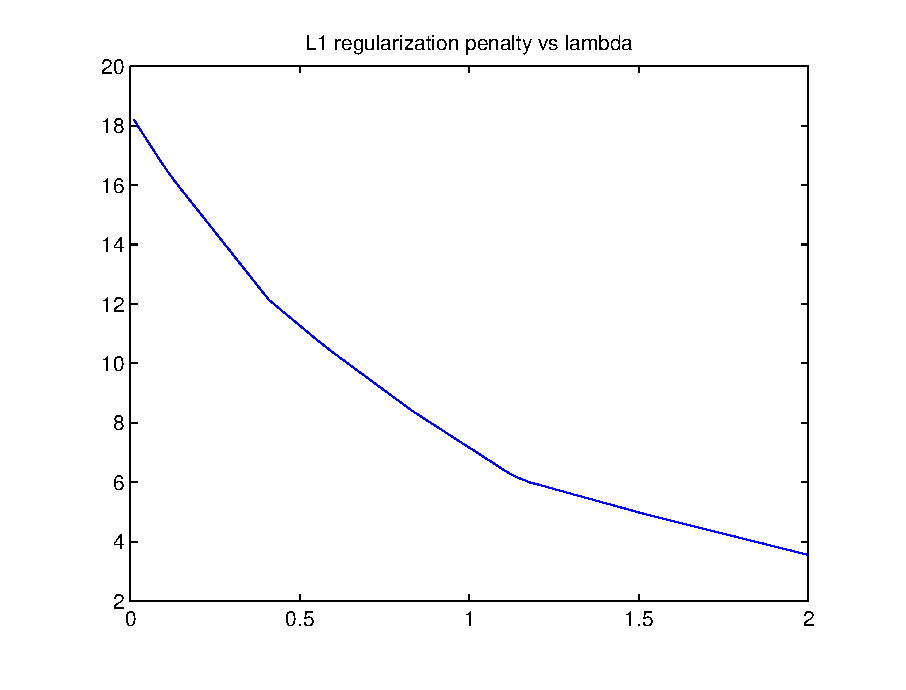
\includegraphics[width=2.2in]{l2.eps}
\end{minipage}
\end{figure}
\begin{figure}[!htbp]
\begin{minipage}[t]{0.3\linewidth}
\centering
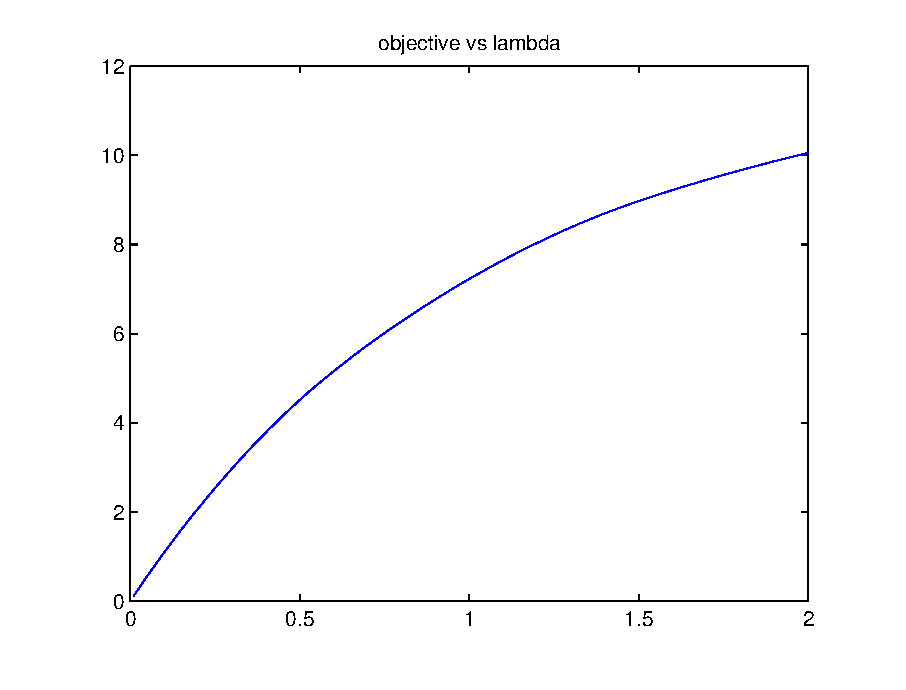
\includegraphics[width=2.2in]{s3.eps}
\end{minipage}%
\begin{minipage}[t]{0.3\linewidth}
\centering
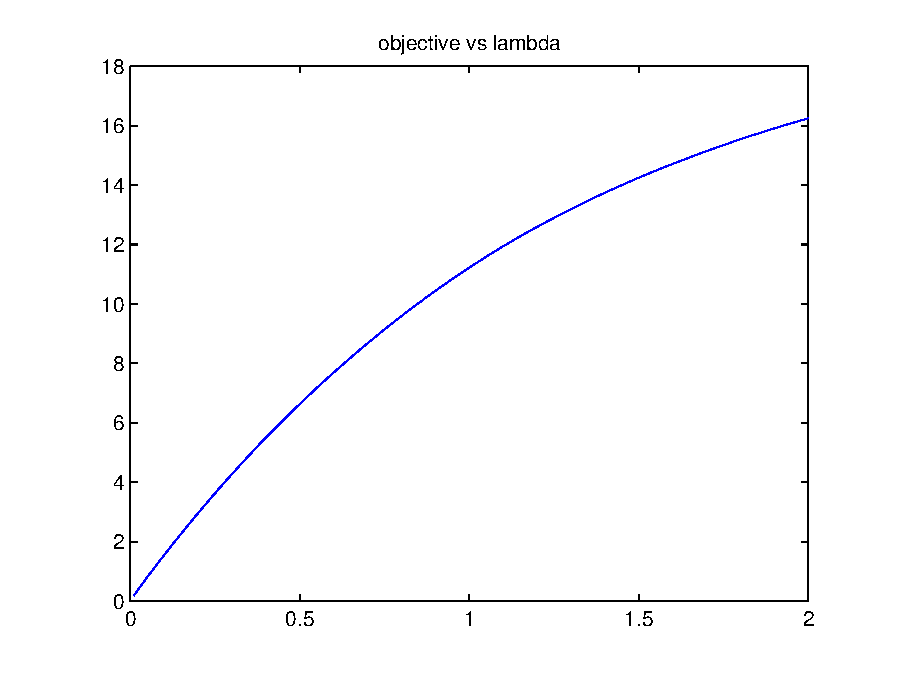
\includegraphics[width=2.2in]{m3.eps}
\end{minipage}
\begin{minipage}[t]{0.3\linewidth}
\centering
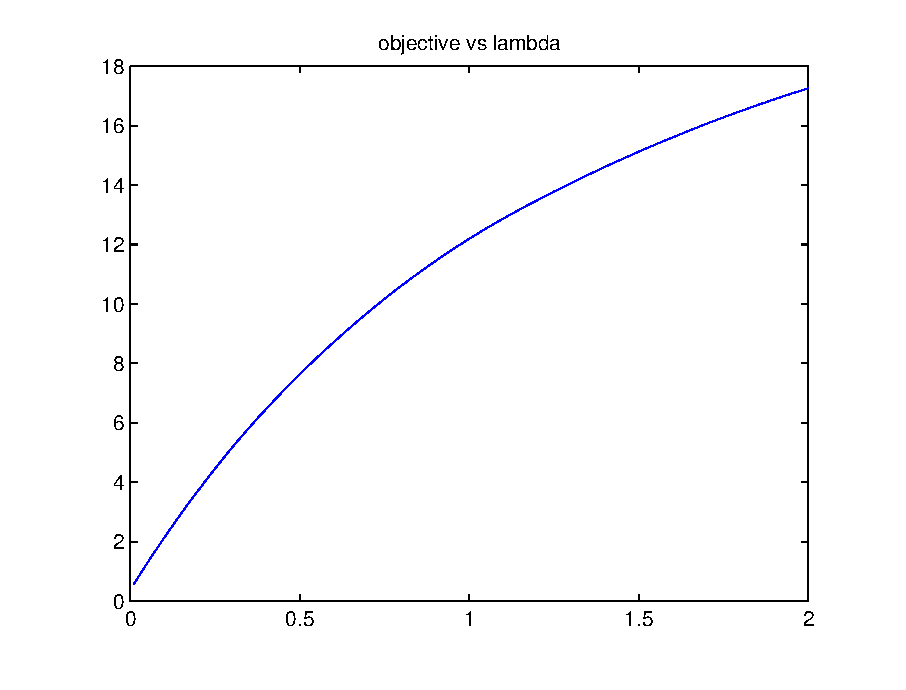
\includegraphics[width=2.2in]{l3.eps}
\end{minipage}
\end{figure}
\begin{figure}[!htbp]
\begin{minipage}[t]{0.3\linewidth}
\centering
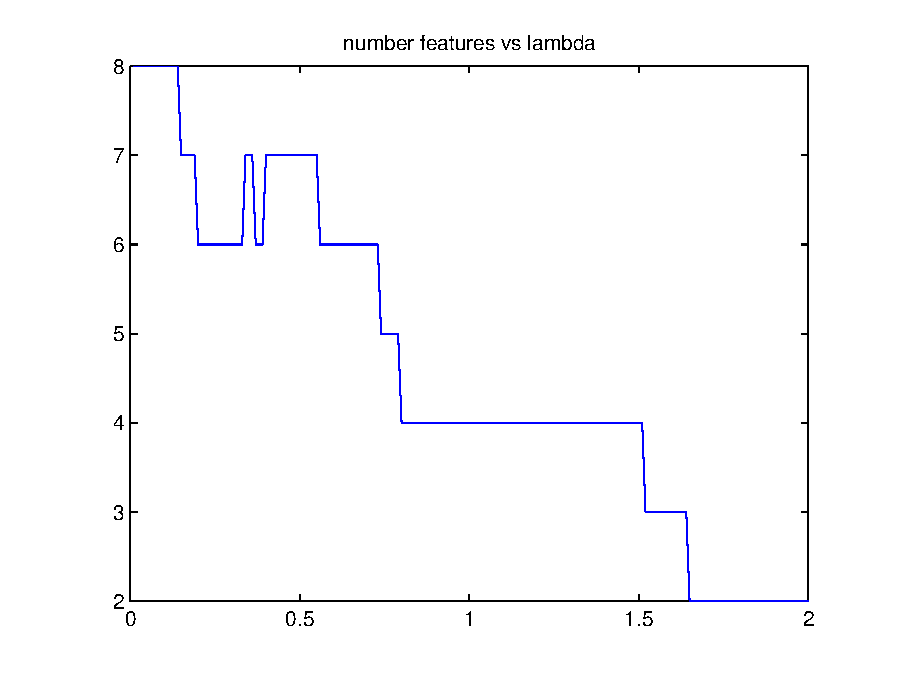
\includegraphics[width=2.2in]{s4.eps}
\end{minipage}%
\begin{minipage}[t]{0.3\linewidth}
\centering
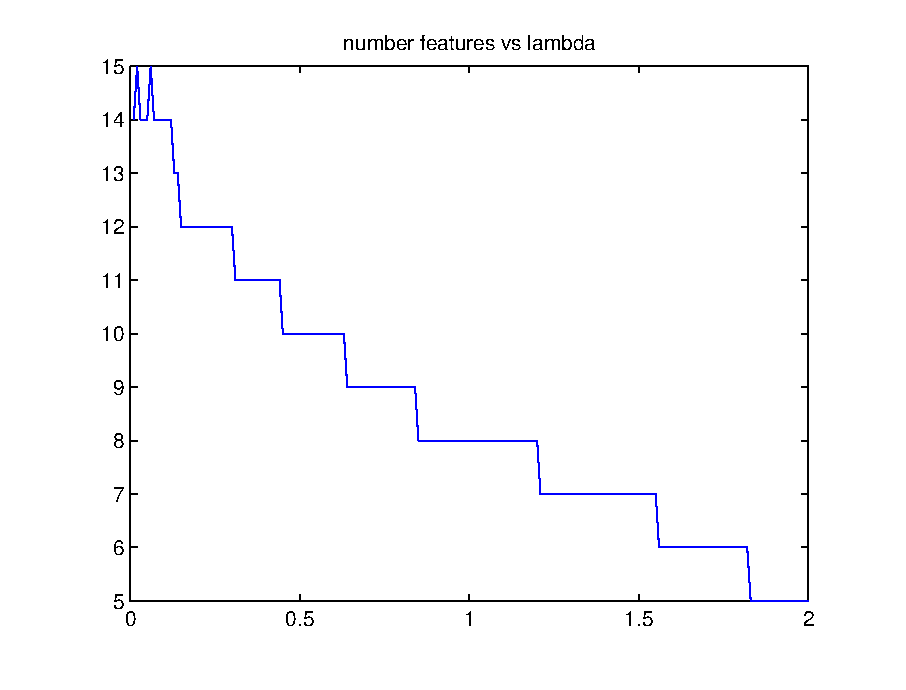
\includegraphics[width=2.2in]{m4.eps}
\end{minipage}
\begin{minipage}[t]{0.3\linewidth}
\centering
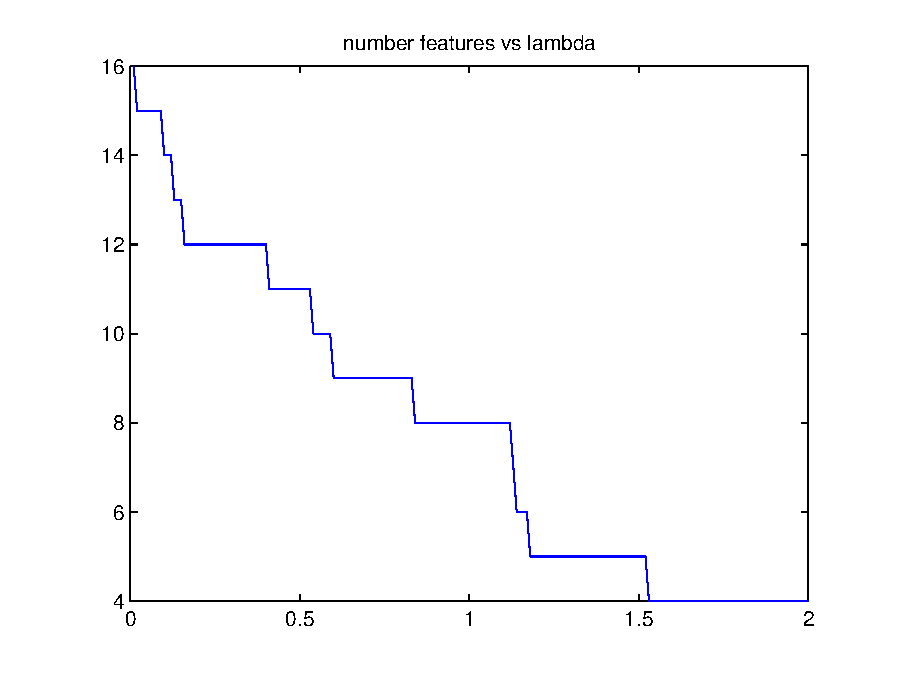
\includegraphics[width=2.2in]{l4.eps}
\end{minipage}
\end{figure}
\begin{figure}[!htbp]
\begin{minipage}[t]{0.3\linewidth}
\centering
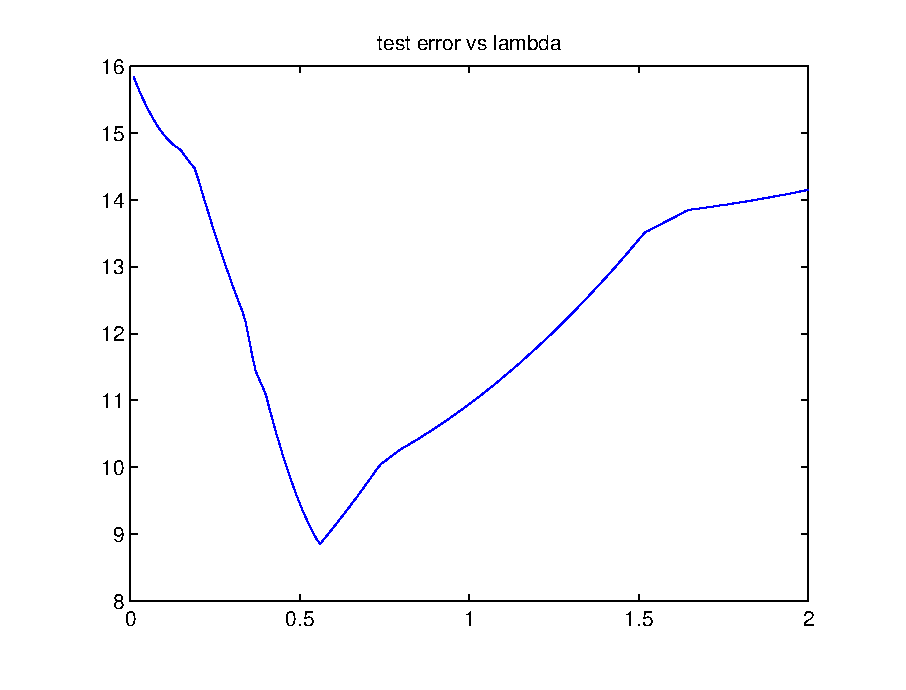
\includegraphics[width=2.2in]{s5.eps}
\caption{Small}
\end{minipage}%
\begin{minipage}[t]{0.3\linewidth}
\centering
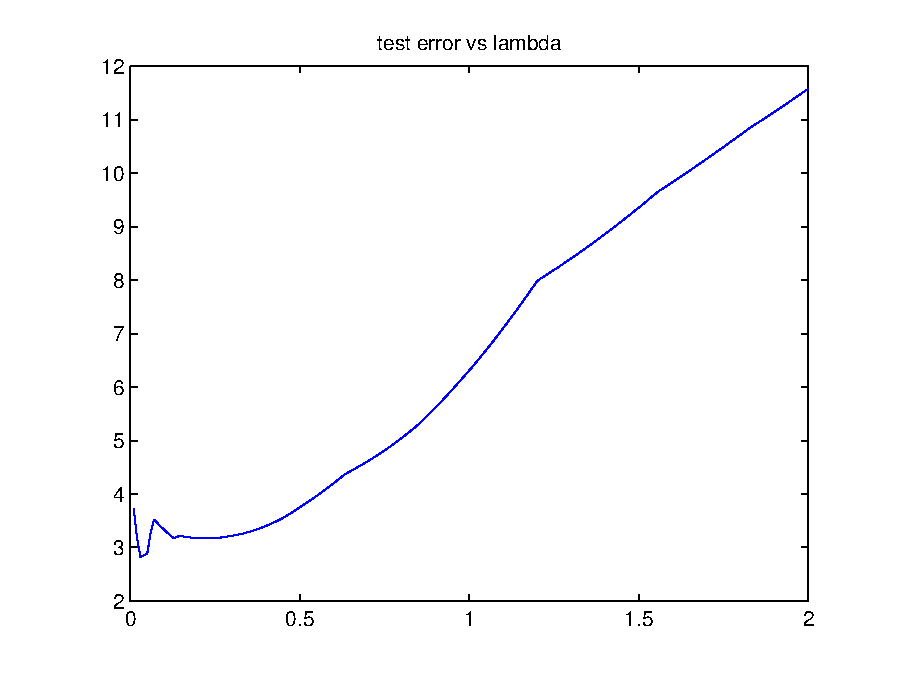
\includegraphics[width=2.2in]{m5.eps}
\caption{Medium}
\end{minipage}
\begin{minipage}[t]{0.3\linewidth}
\centering
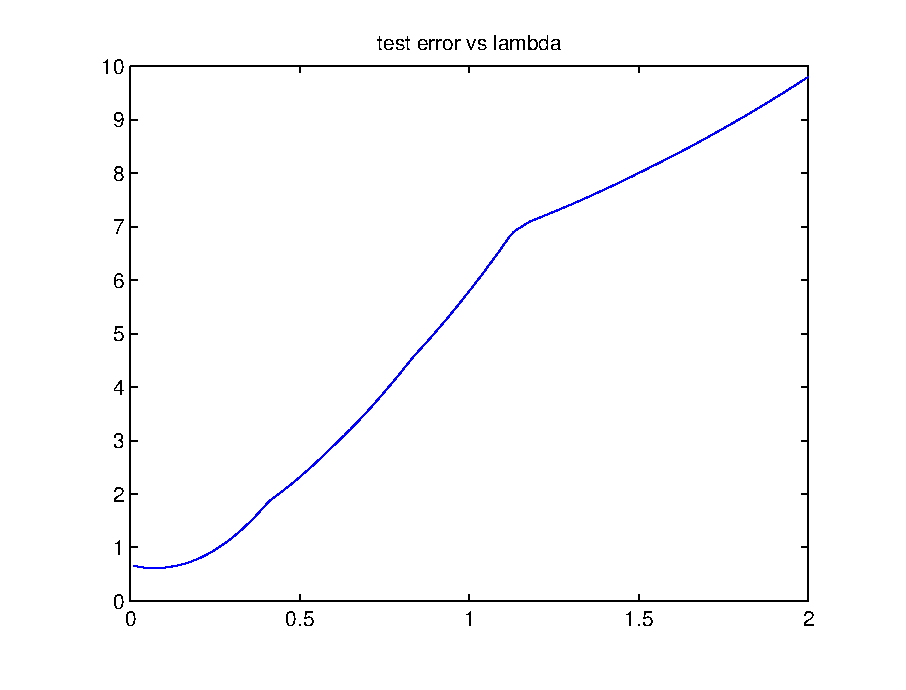
\includegraphics[width=2.2in]{l5.eps}
\caption{Large}
\end{minipage}
\end{figure}
%%%%%%%%%%%%%%%%%%%%%%%%%%%%%%%%%%%%%%%%%%%%%%%%%%%%%%%%%%%%%%%%%%%%
% Reference
%%%%%%%%%%%%%%%%%%%%%%%%%%%%%%%%%%%%%%%%%%%%%%%%%%%%%%%%%%%%%%%%%%%%
%\begin{thebibliography}{1}

%\bibitem{Ray2015}
%Changshui Zhang, \emph{Pattern Recognition}, Tsinghua
%\end{thebibliography}
\end{document}
